\section{The Oculomotor System} \label{sec:bt_TheOculomotorSystem}

Only second to the brain, the human eye is one of the most complex organs in our bodies. Its anatomy has perplexed scientists for centuries, and the mere fact of its complexity was a major argument that Charles Darwin had to circumvent during the making of \textit{On The  Origin of Species} (\cite{oyster1999}). "If a complex mechanical contrivance like a watch requires a watchmaker, something as wonderful as the eye, which is beyond the wit and ability of a man to create, must have an eyemaker". 

What Darwin struggled to explain in 1859 is better understood in the academic community of today, and it is apparent that vision has proved a winning factor in evolution. In fact, zoologists believe that animals where eyes have developed beyond a primitive stage, constitute about 96\% of known living species. Human eyes are inherited from our primate ancestors, and little has changed in terms of general eye composition since we diverged from our most common ancestors about 30 million years ago. The versatility of the human eye in combination with our brain has been one of the driving forces of our rapid cultural evolution. This thesis is mostly concerned with the oculomotor system, an intricate network of muscles and neural circuits that control eye position and in turn determine how humans perceive their environment.
% The final 4\% can be found in environments where light is nonexistent, or in immobile animals where relocation as a response to the detection of light poses no real advantage. This suggests that 

\subsection{Brief Anatomy}
The oculomotor system can not be explained in detail by its components alone. The human eye incorporates several distinct major and minor structures and regions that transform light into perception. However, its macroscopic anatomy is quite simple and readily explainable. As Gordon Walls, a renowned professor of physiological optics and optometry once put it: "The eye is (simply) a fluid-filled chamber enclosed by three coats or layers, of tissue. It is an optical system made of leather, water and jelly" (\cite{oyster1999}), as can be observed by figure \ref{fig:bt_eye}.

Leather would refer to the white \textit{sclera}, a rigid tissue making up most of the outermost coat of the eye, gel-like \textit{vitreous} what makes up most of the interior volume. Light is admitted through and partially refracted by an area at the front of the eye, where the sclera yields to a transparent coat termed the \textit{cornea}. After the cornea, light passes through an aperture stop known as the \textit{pupil}. The pupil is in essence just an opening within the \textit{iris}, a sphincter known for its abundance of melatonin pigments and rich colors which serves to regulate the pupil opening. Light is further refracted in the \textit{lens}, before reaching the \textit{retina} at the very back of the eye. This is where light is processed and transmitted to the brain via millions of very sensitive photoreceptor cells. 

\begin{figure}[h]
    \centering
    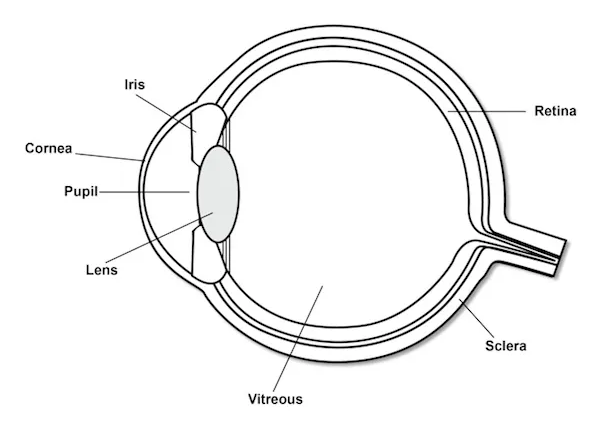
\includegraphics[width=\textwidth]{Images/bt_eye.png}
    \caption{Anatomy of the human eye, in terms of its major and most structures.}
    \label{fig:bt_eye}
\end{figure}

\subsubsection{The Extraocular Muscles}

Central to the oculomotor system are the muscles which allow for physical translation and rotation of the eye in space, in turn enabling the brain to control which parts of the environment it wants to perceive. Movement is enabled by \textit{extraocular} muscles arranged in three agonist-antagonist pairs, meaning there are six muscles in total, each pulling in the opposite direction of another. Together they allow for accurate horizontal and lateral positioning, as well as -90\degree to +90\degree torsions. As muscle fibres are inherently elastic, each extraocular muscle exert passive force even when not actively engaged. This means that for the eye to hold any one stationary position, all six muscles are counterbalanced by an equal and opposite force, producing an equilibrium.

Any particular eye position is dictated by a set extraocular muscle lengths, which in turn is dictated a set of \textit{innervational} commands from the neural circuitry that controls eye movement. For a muscle fibre, its innervation level correspond to the steady-state firing rate of the neural signals to its muscle neuron. 

%Innervation, the process of supplying nerve signals to an organ or part of the body. A particular level of innervation to a muscle always produces the same state of contraction or relaxation and a particular set of innervational commands to the six muscles always produces the same eye position relative to all three axes of rotation.

As we know from mechanics, the acceleration of an object is given by the net sum of its acting forces. As such, the speed of eye movement is given by the change in innervation of the extraocular muscles from one level to another. Slow eye movements can be recognized by gradual changes of a neuron's mean firing rate. Fast movements require a brief high-velocity burst of neural activity which initiates the rapid movement. 
As will be made clear in the following subsection, the human eye is capable of a very wide range of movement velocities, from 0.05\degree to 500\degree per second. Such an enormous range of contraction velocities make the extraocular muscles unique compared to any other muscles in our bodies.

%The speed of eye movement is dictated the change in innervation of the extraocular muscles from one level to another. Every level of innervation in turn dictated by the steady-state firing rate of nerve impulses from each muscles motor nerve. Slow eye movements (e.g. smooth pursuit) can be recognized by gradual changes of a neuron's mean firing rate. Fast movements (saccades) require a brief high-frequency burst of neural activity that produce forces which initiates the rapid eye movement.

\subsection{Eye Movement}
Since most photoreceptors of the retina are concentrated at the fovea, a tiny 1.5mm wide pit right behind the lens, there is only a tiny area in the field of view which provide clear vision. As we will see, eye movements are therefore crucial not only to move the field of view between areas of interest, but also for image stabilization, focus and more. This gives rise to the need for complex patterns of eye movement, some of which will be mentioned here.

\textit{Saccades are neccessary to place AOI at the center of the fovea, where the photoreceptors are most tightly packed. Saccade durations rarely more than 50ms. Post-saccadic oscillations. Speeds of up to 500\degree/s. Vision is suppressed during saccade.}

\textit{miniature eye movements during fixations}

\textit{Slow eye movements are necessary to keep AOI at the center of the fovea during cases where the object to be kept stable on the fovea while moving. e.g. head movement, target tracking (smooth pursuit). Speeds of 0.05\degree/s-20\degree/s. Max up to 90\degree/s.}

\textit{The overlapping fields of view of two eyes. Constitute vergence, another eye movement type which is necessary to place objects in plane of focus. Slow movements, up to 30 \degree/s. Under everyday conditions, other eye movements are generally superimposed on vergences.}

\textit{Although the eye is not particularly heavy (7.5g in adults), its mass does pertain a tiny bit of inertia which resists movement. This inertia is what constitutes the rapid increase in neural activity required for rapid eye movements, as well as some oscillations often observed following a saccade. Post-saccadic oscillations.}

\textit{Eye movements translated to on-screen coordinates? Find sources. Tobii?}








